\begin{subsection}{Plataforma Cloud}
    A lo largo de esta sección se mostrará la configuración establecida en vRA y cómo los usuarios del entorno de pruebas utilizan la plataforma Cloud. Primero se habilitarán los recursos necesarios para que luego los usuarios los aprovisionen mediante la creación de dos proyectos. 

    \begin{subsubsection}{Preparación de los recursos}
    El aprovisionamiento de recursos con vRA se traduce en la creación de VMs a partir de plantillas creadas previamente por el administrador, y al uso de las subredes y almacenamiento que se encuentran disponibles en el entorno. Con el objetivo de organizar las VMs creadas por los usuarios, en el cluster vSphere situado en la instancia de VMware vCenter Server descrita anteriormente, se crean una carpeta y un \textit{resource pool} donde se desplegarán las nuevas VMs como se muestra en la siguiente figura.
    \begin{figure}[h]
        \centering
        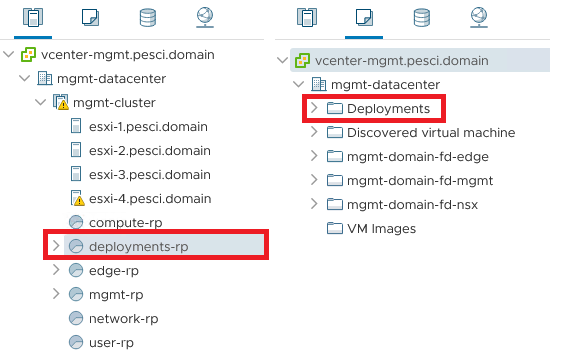
\includegraphics[width=0.4\textwidth]{imaxes/pruebaconcepto/vrealize/rp-vra.png}
        \caption{\textit{Resource pool} (izquierda) y carpeta (derecha) creadas para alojar las VMs desplegadas desde vRA.}
        \label{fig:rp-folder-vra}
    \end{figure}
    \FloatBarrier
    % Para que las VMs creadas por los usuarios tengan acceso a la red, se crea un nuevo Segment en el router virtual Tier-1 de VMware NSX-T (Figura \ref{fig:two-tier-topology}) donde se alojará una subred dedicada exclusivamente a ser consumida por los usuarios. Al generar el Segment los componentes de VMware NSX-T comunican al router VyOS la nueva ruta mediante el protocolo de enrutamiento BGP, por lo tanto no es necesario aplicar ninguna configuración adicional en los recursos de red físicos.
    Para que las VMs creadas por los usuarios tengan acceso a la red, se utilizará el Segment \textit{mgmt-Region01A-VXLAN} disponible en VMware NSX-T (Figura \ref{fig:two-tier-topology}). Se configura además un servidor DHCP dentro de VMware NSX-T y así poder establecer la configuración IP de forma automática a cada nueva VM que se conecte a la subred contenida en el Segment. 
    \begin{figure}[h]
        \centering
        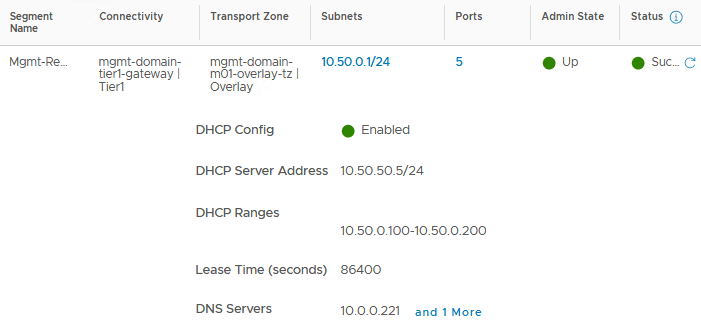
\includegraphics[width=0.4\textwidth]{imaxes/pruebaconcepto/vrealize/segment-MGMT.png}
        \caption{Segment utilizado para el despliegue de VMs con vRA (arriba) y la configuración del servidor DHCP definida en VMware NSX-T (abajo)}
        \label{fig:topology-segment-mgmt}
    \end{figure}
    \FloatBarrier
    % \begin{figure}[h]
    %     \centering
    %     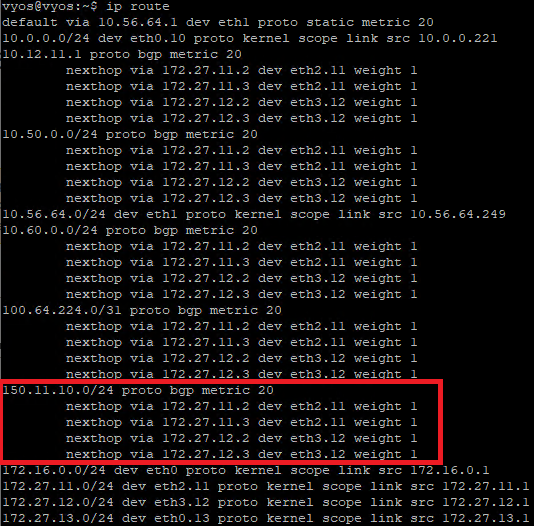
\includegraphics[width=0.4\textwidth]{imaxes/pruebaconcepto/vrealize/router-vyos-bgp.png}
    %     \caption{Nueva ruta configurada en el router VyOS mediante BGP.}
    %     \label{fig:bgp-router-vyos}
    % \end{figure}
    % \FloatBarrier    
    Las plantillas empleadas por los usuarios para generar VMs son generadas por el administrador del SDDC. Para crear una plantilla el administrador debe antes crear una VM, instalar en ella el sistema operativo deseado y establecer una configuración inicial. En el entorno de pruebas, dentro del cluster vSphere, se crea una VM con el sistema operativo Ubuntu Server 18.04, para inicializarla se instalan las actualizaciones correspondientes y se configura el servicio \textbf{cloud-init}, el cual permitirá al usuario especificar comandos en el diseño para inicializar automaticamente una VM con los requisitos que desee (instalación de paquetes, creación de usuarios, generación de claves SSH, configuración de red y mucho más\footnote{En el siguiente enlace se pueden encontrar más información sobre cloud-init y ejemplos sobre sus usos: \url{https://cloudinit.readthedocs.io/en/latest/topics/examples.html}}). Una vez configurada se procede a ejecutar un script\footnote{El script se puede encontrar en el anexo .} para limpiar la VM para que cada vez que se utilice la plantilla se genere una VM distinta. Finalmente la VM se convierte a una plantilla que se almacena en VMware vCenter Server. 
    % Siguiendo un procedimiento similar se crea una plantilla a partir de una VM con Windows Server 2016 y otra plantilla con CentOS 8.
    \begin{figure}[h]
        \centering
        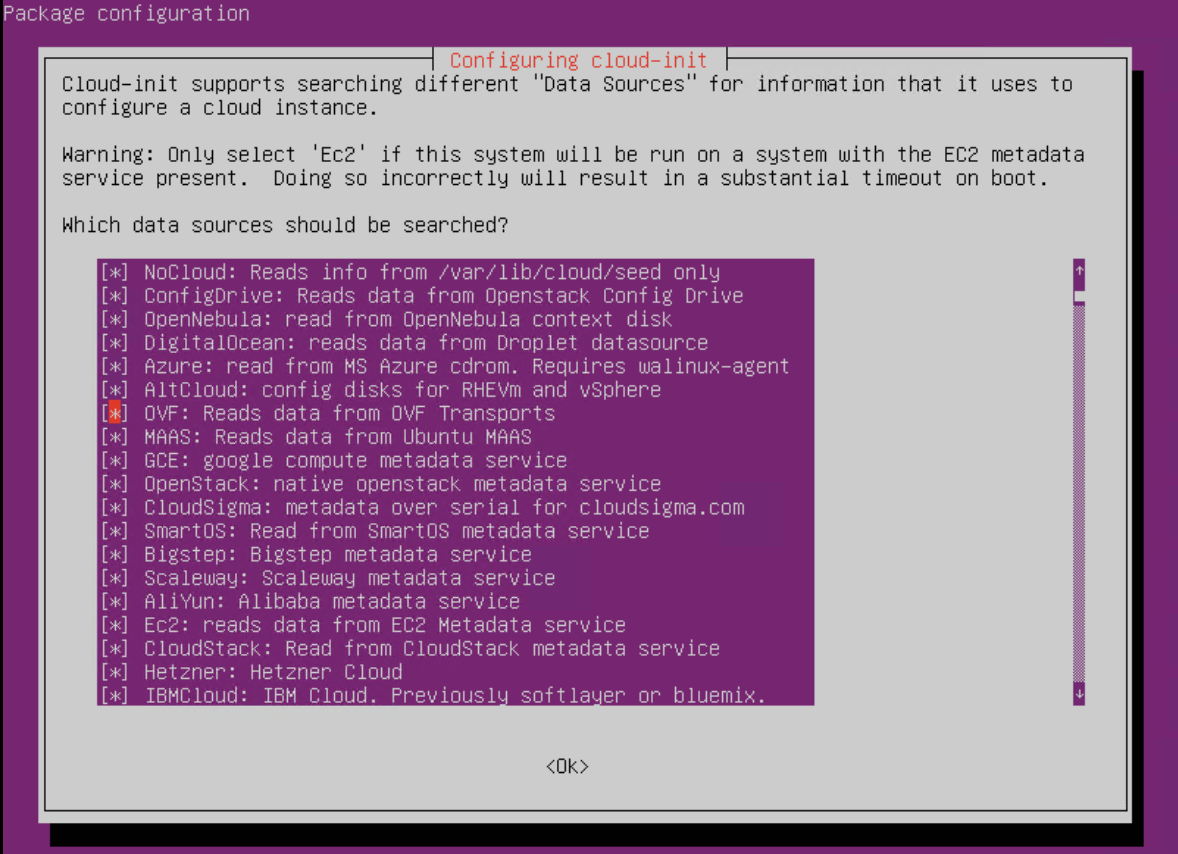
\includegraphics[width=0.6\textwidth]{imaxes/pruebaconcepto/vrealize/install-cloud-init.png}
        \caption{Configuración del servicio cloud-init en Ubuntu Server 20.04.}
        \label{fig:cloud-init-config}
    \end{figure}
    \FloatBarrier
    \begin{figure}[h]
        \centering
        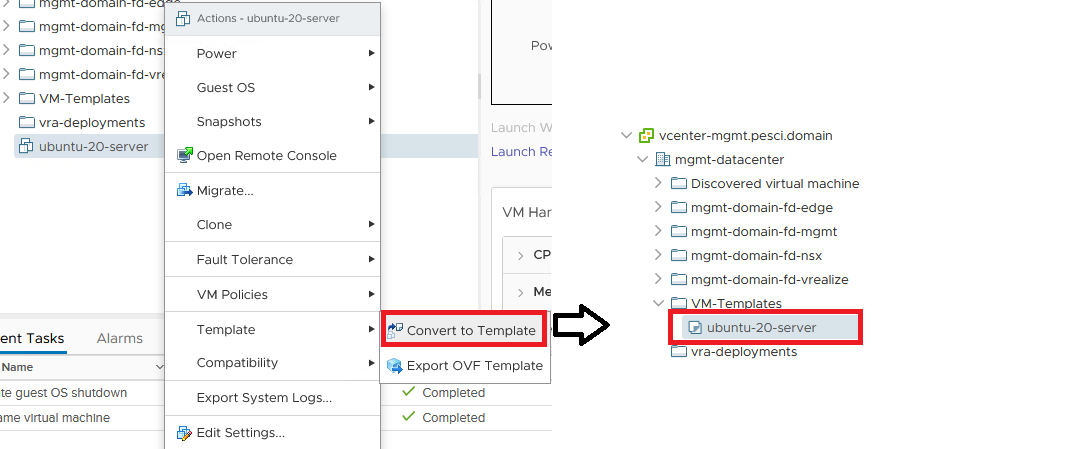
\includegraphics[width=0.6\textwidth]{imaxes/pruebaconcepto/vrealize/convert-to-template-Ubuntu.png}
        \caption{Creación de una plantilla a partir de la VM de Ubuntu Server 18.04.}
        \label{fig:template-ubuntu}
    \end{figure}
    \FloatBarrier
    Se crea otra VM con el sistema operativo Windows Server 2016. En este caso, en lugar de cloud-init se utiliza el servicio \textit{cloudbase-init}\footnote{La documentación de cloudbase-init se puede encontrar aquí: \url{https://cloudbase.it/cloudbase-init/}} que cumple la misma función que el anterior. Una vez completada la instalación y configuración de Windows Server 2016, desde VMware vCenter Server se convierte la VM en una plantilla.
    \begin{figure}[h]
        \centering
        \includegraphics[width=0.6\textwidth]{imaxes/pruebaconcepto/vrealize/instalación-cloudbase-windows.png.png}
        \caption{instalación de cloudbase-init en Windows Server 2016.}
        \label{fig:cloudbase-init}
    \end{figure}
    \FloatBarrier 

    \end{subsubsection}

    \begin{subsubsection}{Configuración de VMware vRealize Automation}
        Una vez creados los recursos es necesario integrarlos en vRA. A medida que se configuran se asignan los tags necesarios para identificar cada recurso posteriormente.
        En la siguiente imagen se muestran las plantillas creadas anteriormente configuradas en vRA para que los usuarios puedan acceder a ellas.
        \begin{figure}[h]
            \centering
            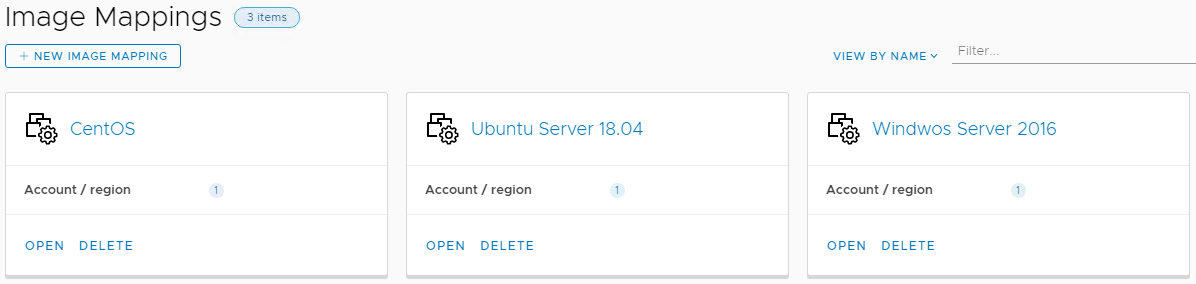
\includegraphics[width=0.6\textwidth]{imaxes/pruebaconcepto/vrealize/image-mappings.png}
            \caption{Plantillas configuradas en vRA.}
            \label{fig:image-mapping}
        \end{figure}
        \FloatBarrier
        El Segment configurado en VMware NSX-T se añade como un perfil de red en vRA. Este Segment contiene un servidor DHCP configurado, pero existe la posibilidad de crear un rango de direcciones IP para asignar una IP estática a cada VM que utiliza este perfil. A la subred se le han asignado los tags \textit{subnet-cidr:10.50.0.0/24}, \textit{function:pro} y \textit{env:pro}.
        % , pero en este caso se utiEn este perfil se ha creado un rango de direcciones IP para que vRA asigne una dirección estática a cada VM que lo utilice, y se le han asignado los tags \textit{function: pro} y \textit{env: pro}.
        \begin{figure}[h]
            \centering
            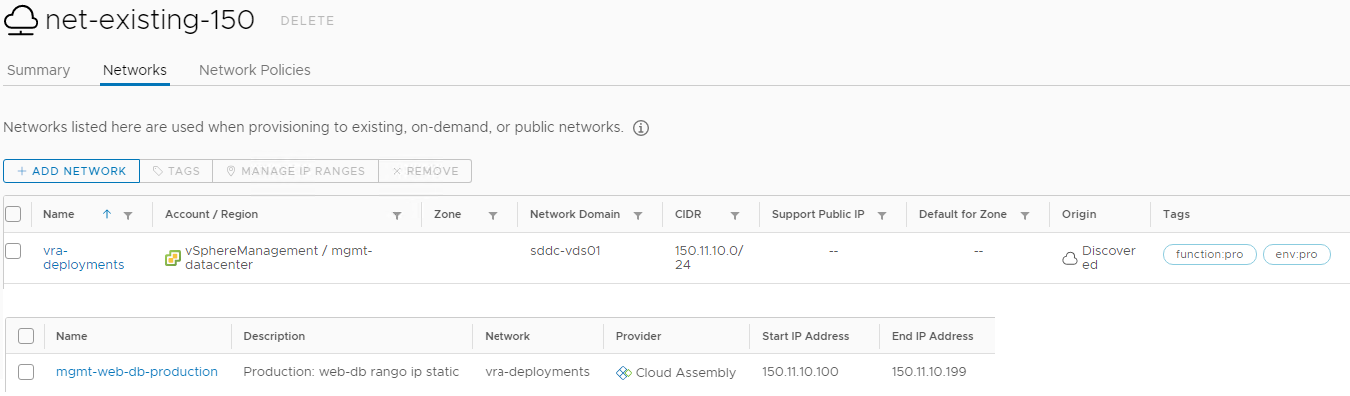
\includegraphics[width=0.6\textwidth]{imaxes/pruebaconcepto/vrealize/net-profile.png}
            \caption{Perfil de red creado en vRA con el Segment generado en VMware NSX-T.}
            \label{fig:net-profile}
        \end{figure}
        \FloatBarrier
        Los recursos de cómputo se habilitan a través de la Cloud Zone que se muestra en la siguiente imagen. Esta utiliza los recursos del cluster vSphere mencionado, establece la política a seguir para elegir el host donde se debe desplegar cada VM (la opción DEFAULT escoge un host aleatoriamente) y la carpeta de VMware vCenter Server donde se deben colocar las VMs. A esta Cloud Zone se le han asignado los tags \textit{cloud: private} y \textit{region: management}. Además, se le asigna el tag \textit{resource: rpprivate} al resource pool configurado previamente para poder colocar en él las VMs creadas
       \begin{figure}[h]
            \centering
            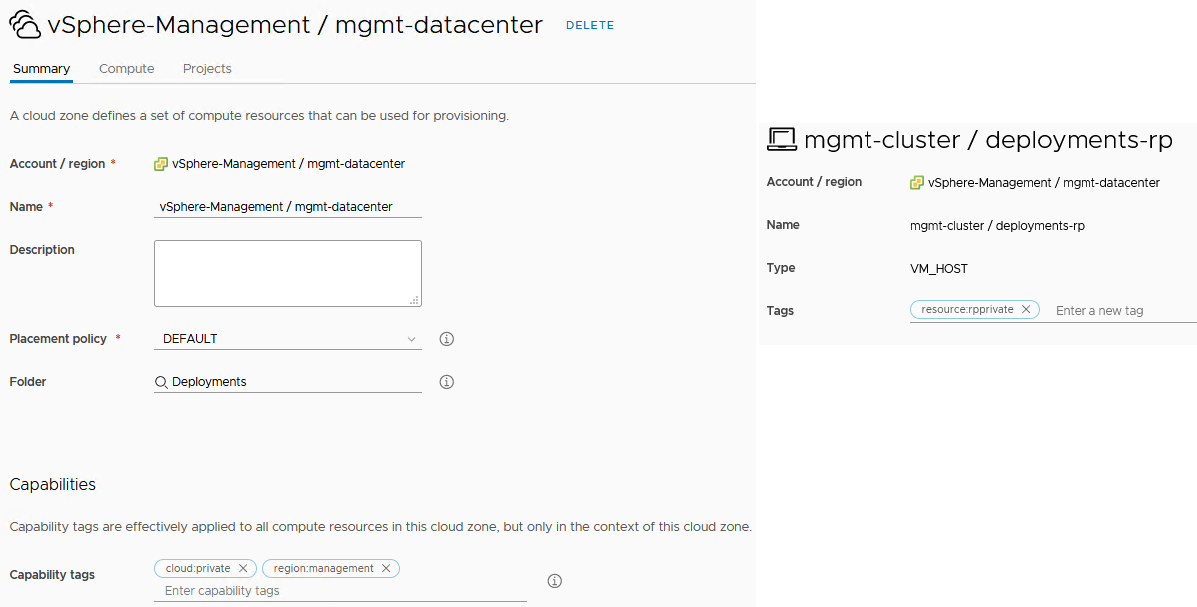
\includegraphics[width=0.6\textwidth]{imaxes/pruebaconcepto/vrealize/cloud-zone.png}
            \caption{Cloud Zone (izquierda) y resource pool (derecha) configuradas para desplegar VMs a través de vRA.}
            \label{fig:cloud-zone}
        \end{figure}
        \FloatBarrier
        Para el almacenamiento, se crea un perfil que se muestra en la siguiente imagen. Este perfil tiene como recurso de almacenamiento el datastore configurado para el Management Domain, y se establece como el perfil por defecto para el aprovisionamiento de recursos de almacenamiento. Se la han asignado los tags \textit{cloud: private} y \textit{function: pro}. 
        \begin{figure}[h]
            \centering
            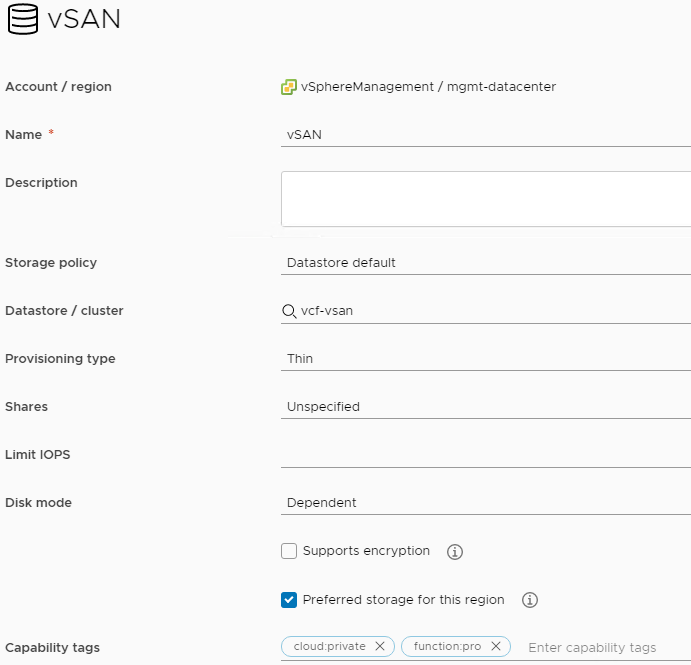
\includegraphics[width=0.6\textwidth]{imaxes/pruebaconcepto/vrealize/datastore-policy.png}
            \caption{Perfil de almacenamiento configurado donde indica el datastore que deben utilizar las VMs.}
            \label{fig:storage-policy}
        \end{figure}
        \FloatBarrier
        Finalmente se configuran los perfiles donde se predefinen los tamaños que la VM creada por un usuario puede tomar. En cada perfil se establece la cantidad de CPU y memoria RAM que se asigna a una VM. Estos tamaños van desde \textit{x-small} con 1 CPU y 512 MB de memoria RAM, hasta \textit{large} con 8 CPUs y 16 GB de memoria RAM.
        \begin{figure}[h]
            \centering
            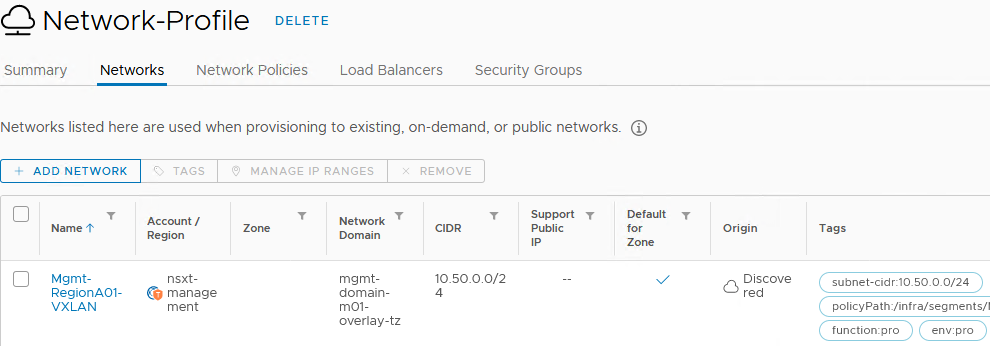
\includegraphics[width=0.6\textwidth]{imaxes/pruebaconcepto/vrealize/falvor-mapping.png}
            \caption{Tamaños preestablecidos para determinar la cantidad de recursos de cada VM.}
            \label{fig:falvor-mapping}
        \end{figure}
        \FloatBarrier

    \end{subsubsection}

    \begin{subsubsection}{Uso de la plataforma}
        La plataforma ya está lista para ser utilizada por los usuarios. Los usuarios del CITIC que utilizarán esta plataforma Cloud están organizados en proyectos, donde existe al menos un coordinador o jefe de proyecto. Cuando un grupo de usuarios quiere utilizar el servicio Cloud primero debe comunicarlo al administrador, el cual crea el proyecto correspondiente y habilita el acceso a cada usuario con sus correspondientes permisos. 
        Como ya se ha visto en la sección \refname{subsubsec:WSA}, en el entorno de pruebas se han configurado cinco usuarios que están divididos en dos proyectos, uno llamado Web-DB con el objetivo de construir una página web con una base de datos y otro llamado Server-Desktop con la idea de crear una VM con Windows Server y otra con CentOS para futuros trabajos. Tomando los usuarios que se muestran en la figura \ref{fig:users-defined-WSA}, el proyecto Web-DB lo forman el usuario \textit{User One}, \textit{User Two} y \textit{Manager One}, el cual es el coordinador del grupo, y el proyecto Desktop-Server está formado por \textit{User Two}, \textit{User Three} y \textit{Manager Two}, el cual será el coordinador de este segundo grupo. Entonces, a los usuarios \textit{Manager One} y \textit{Manager Two} se les asigna el rol Administrador de Proyecto, y al resto de usuarios el rol Miembro de Proyecto, los primeros podrán controlar las blueprints disponibles en el catálogo del proyecto y los usuarios que tienen acceso, mientras que los miembros del proyecto podrán desplegar los diseños habilitados.
        \begin{figure}[h]
            \centering
            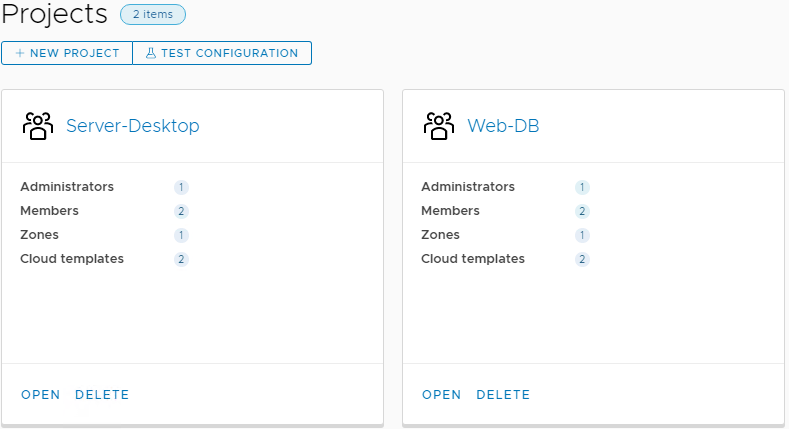
\includegraphics[width=0.6\textwidth]{imaxes/pruebaconcepto/vrealize/projects-vRA.png}
            \caption{Proyectos creados para dar acceso a los usuarios a vRA.}
            \label{fig:projects-vra}
        \end{figure}
        \FloatBarrier
        \begin{figure}[h]
            \centering
            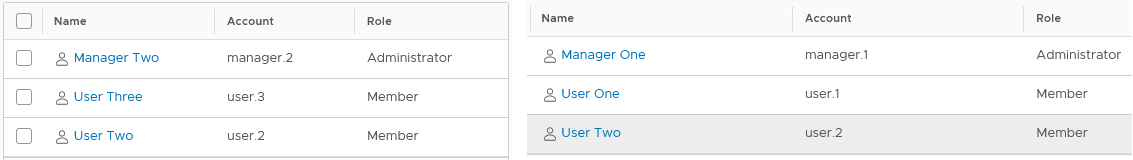
\includegraphics[width=0.6\textwidth]{imaxes/pruebaconcepto/vrealize/users-DB.png}
            \caption{Usuarios del proyecto Server-Desktop (izquierda) y usuarios del proyecto Web-DB (derecha).}
            \label{fig:project-users}
        \end{figure}
        \FloatBarrier
        En cada uno de los proyectos el administrador establece la cantidad máxima de CPU, memoria RAM y almacenamiento que pueden consumir en total los usuarios del proyecto. Como se trata de un entorno de pruebas en el proyecto Server-Desktop se establece un límite de 2 VMs, 10 GB de memoria RAM y 6 CPUs, y en el proyecto Web-DB un límite de 2 VMs, 10 GB de memoria RAM y 6 CPUs, de esta forma los usuarios del proyecto no podrán superar ninguno de los límites establecidos.
        % Cuando el administrador crea un proyecto establece la cantidad máxima de CPU, memoria RAM y almacenamiento que puede consumir en total. También se pueden establecer mediante el uso de tags, los recursos que los despliegues del proyecto deben utilizar por defecto.
        [Foto consumo total]
        
        Para valorar el consumo de recursos de cada proyecto vRA permite establecer un precio al uso de CPU, memoria y almacenamiento.

        Una vez configurados los dos proyectos los usuarios administradores de cada uno pueden acceder y empezar a crear los diseños de los recursos que quieran aprovisionar. El coordinador del proyecto Server-Desktop, \textit{Manager Two}, a través de Cloud Assembly crea el diseño que se muestra en la siguiente imagen\footnote{En el anexo \ref{appendix:wd-server-blueprint} se encuentra el contenido del archivo .yaml donde se establece la configuración del diseño.}.
        \begin{figure}[h]
            \centering
            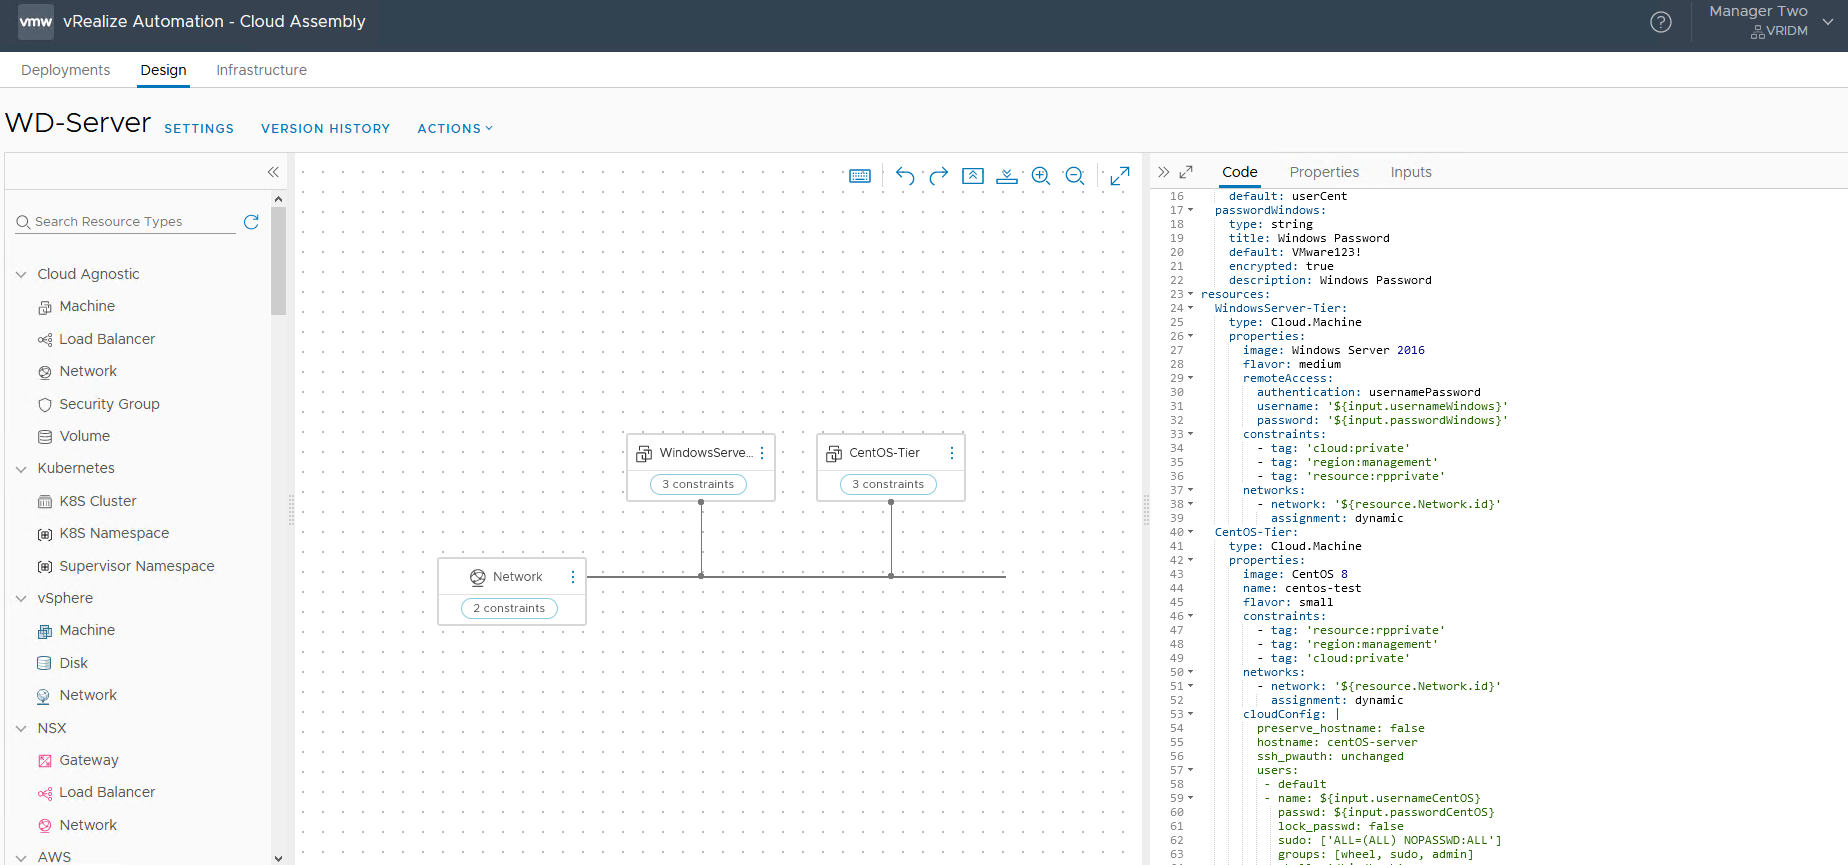
\includegraphics[width=0.6\textwidth]{imaxes/pruebaconcepto/vrealize/windows-centos-blueprint.png}
            \caption{Diseño WD-Server para proyecto Server-Desktop.}
            \label{fig:server-desktop-blueprint}
        \end{figure}
        \FloatBarrier
        En este diseño se define una VM con el sistema operativo Windows Server 2016 y otra con CentOS 8, ambas VMs se conectan a una red que también se define en el diseño. Se establecen además unas credenciales para cada VM, cuyos datos son introducidos por el usuario cuando se despliega el diseño y así poder iniciar sesión en ellas mediante SSH. Los tags que se utilizan en la definición de las VMs son \textit{cloud:private}, \textit{region:management} y \textit{resource:rpprivate}, y el tag \textit{subnet-cidr:10.50.0.0/24} en la definición de la red, por lo tanto ambas VMs utilizarán los recursos del cluster vSphere y el Segment definido en VMware NSX-T. En cuanto a la configuración de las interfaces de red, se puede establecer una configuración de forma estática pero como en la subred utilizada existe un servidor DHCP, entonces se aplicará de forma dinámica. Una vez completado el diseño, \textit{Manager Two} publica el diseño en el catálogo del proyecto para que los usuarios puedan acceder a él. Durante la publicación se especifica la versión del diseño ya que este puede ser actualizado.
        \begin{figure}[h]
            \centering
            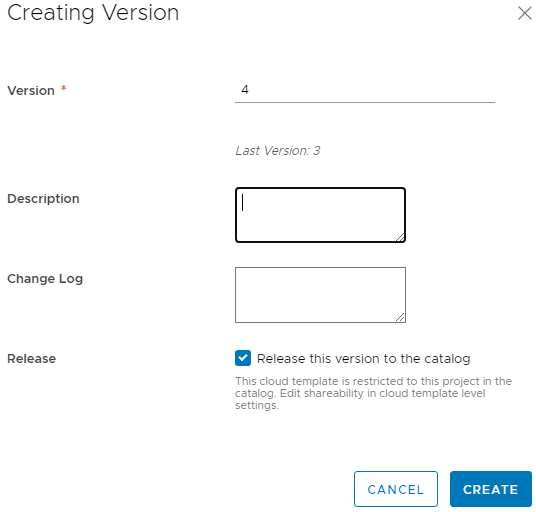
\includegraphics[width=0.6\textwidth]{imaxes/pruebaconcepto/vrealize/create-version-blueprint.png}
            \caption{Publicación en el catálogo de una nueva versión del diseño.}
            \label{fig:publication-version}
        \end{figure}
        \FloatBarrier

        De la misma forma que para el proyecto Server-Desktop, el coordinador del proyecto Web-WD, \textit{Manager One}, crea el diseño de los recursos necesarios para que los usuarios del proyecto puedan generar un sitio web basado en Wordpress, con el objetivo de que una vez desplegados los recursos el usuario pueda trabajar inmediatamente en su página web sin ocuparse de la configuración el entorno. En la siguiente imagen se muestra el diseño creado para el proyecto Web-WD\footnote{En el anexo \ref{appendix:worpress-mysql-blueprint} se encuentra el contenido del archivo .yaml donde se establece la configuración del diseño.}.
        \begin{figure}[h]
            \centering
            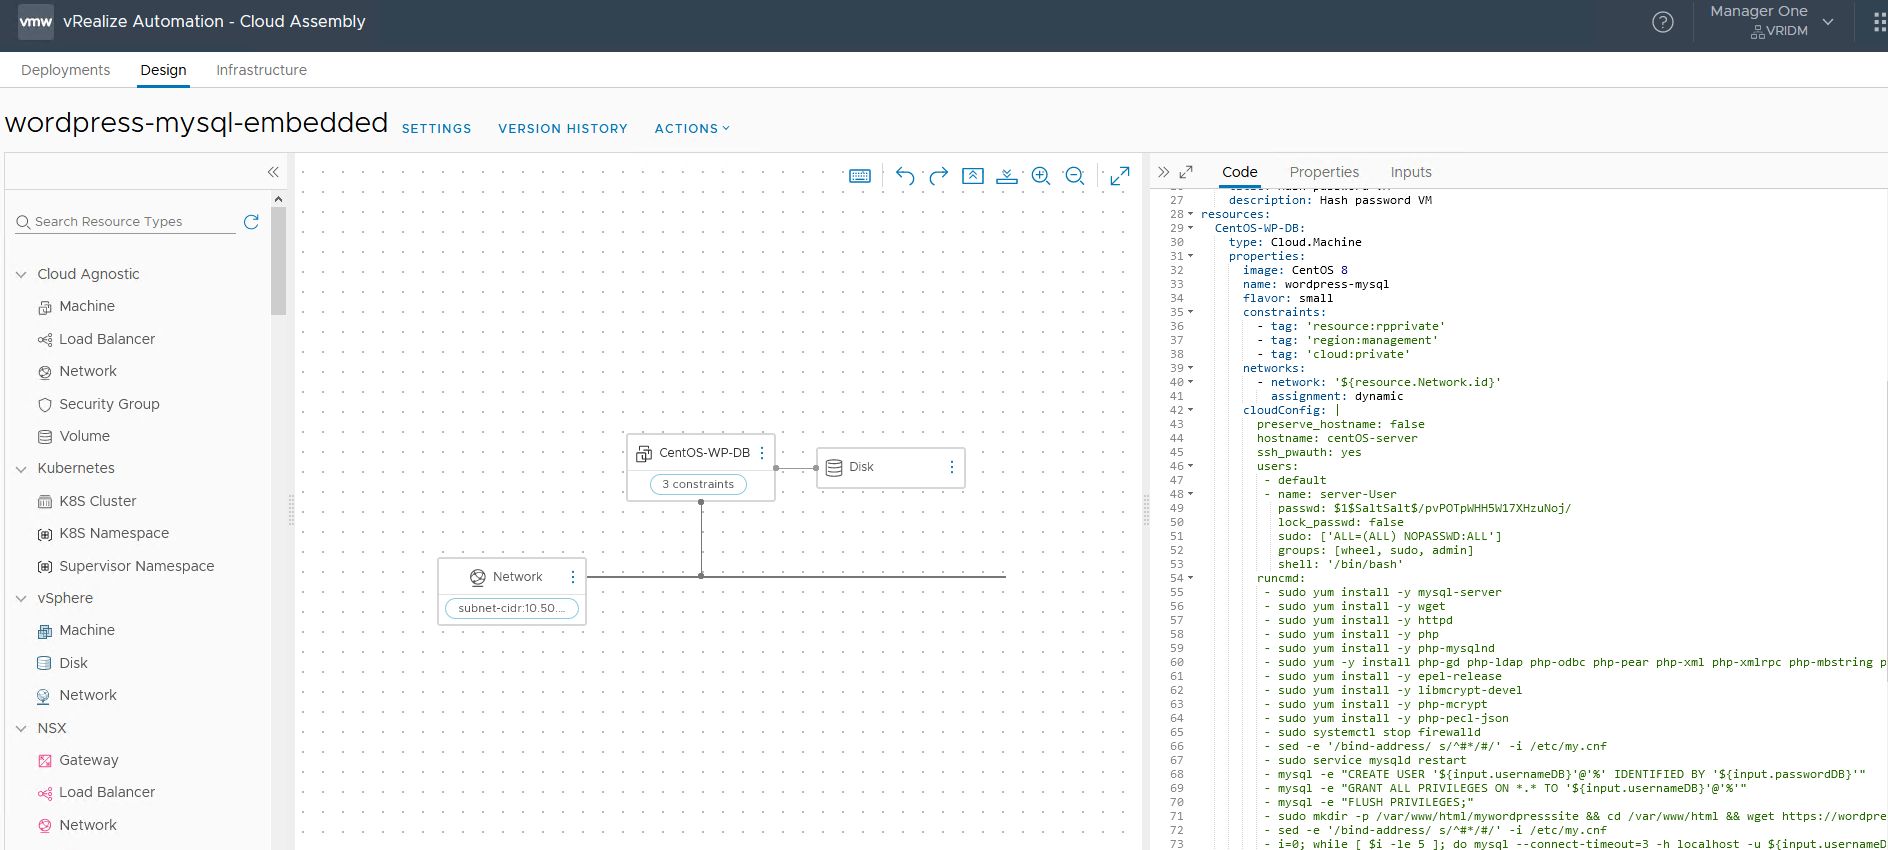
\includegraphics[width=0.6\textwidth]{imaxes/pruebaconcepto/vrealize/wordpress-mysql-blueprint.png}
            \caption{Diseño Wordpress-MySQL-Embedded para el proyecto Web-WD.}
            \label{fig:web-WD-blueprint}
        \end{figure}
        \FloatBarrier
        En este diseño se define una VM con el sistema operativo CentOS 8, la cual se conecta a una red y se le añade un disco de almacenamiento. Durante el despliegue del diseño, en la VM se instala y configura el gestor de base de datos MySQL y el framework web Wordpress. Para ello, se hace uso de la propiedad \textbf{cloudConfig} la cual invoca al servicio \textbf{cloud-init} para la ejecución de los comandos definidos en el diseño, que en este caso se utilizan para descargar los paquetes de MySQL, Wordpress y sus dependencias, y posteriormente crear una base datos, configurar Wordpress para conectarse a ella y habilitar un servidor Apache para acceder al sitio web. 
        
       
        % Desde el componente Cloud Assembly de vRA, el administrador crea los dos proyectos y asigna respectivamente el rol Administrador de Poryecto a los usuarios \textit{Manager One} y \textit{Manager Two}, mientras que el resto de usuarios reciben el rol Miembro de Proyecto. Con esta asignación cada usuario solo podrá acceder a los proyectos donde se le haya asignado un rol, lo cual podrán hacer a través del componente Service Broker de vRA.
        % El administrador de cada proyecto se encargará del diseño de blueprints, de habilitar las blueprints en el catálogo del proyecto y de controlar los usuarios que son miembros del proyecto. Los miembros del proyecto podrán realizar despliegues a partir de las blueprints habilitadas por el administrador del proyecto. 
        
    \end{subsubsection}

    % Para ordenar el aprovisionamiento de los recursos, antes de realizar cualquier implementación, es necesario configurar la infraestructura que se va a poner a disposición de los usuarios. 
    %     En VMware vCenter Server, dentro del cluster vSphere se define un \textit{resource pool} y una carpeta que se utilizarán para colocar las VMs que se desplieguen desde vRA. 
    %     La red que utilizarán las VMs generadas estará controlada por VMware NSX-T para aprovechar las ventajas de sus redes definidas por software y así automatizar su configuración y hacer uso de los servicios que ofrece. Para ello se añade un Segment al router virtual de Tier-1 que se muestra en la figura \ref{fig:two-tier-topology}, VMware NSX-T informa de la nueva ruta al router físico mediante BGP proporcionando así acceso a redes externas.
    %     \begin{figure}[h]
    %         \centering
    %         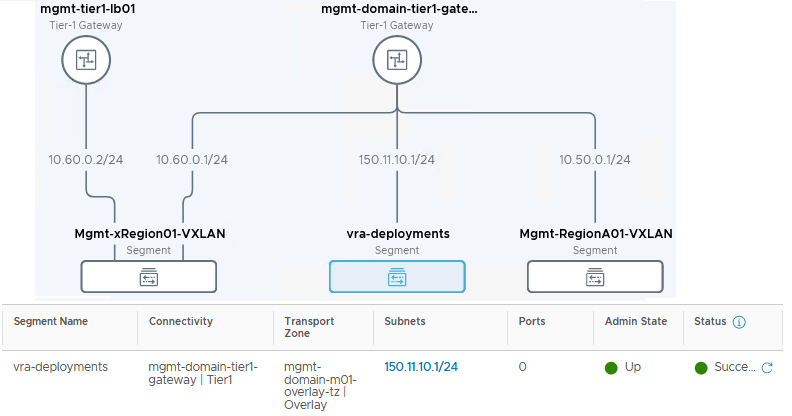
\includegraphics[width=0.4\textwidth]{imaxes/pruebaconcepto/vrealize/topology-for-vRA-NSXT.png}
    %         \caption{Nuevo Segment \textit{vra-deployments} en el router virtual Tier-1.}
    %         \label{fig:topology-nsx-t-vra}
    %     \end{figure}
    %     \FloatBarrier
    %     Las VMs que los usuarios generan están basadas en plantillas que son creadas previamente por el administrador. Antes de generar la plantilla el administrador debe crear una VM en VMware vCenter Server y proveerla con una configuración mínima para que el usuario pueda aplicar su propia configuración durante el despliegue, para este entorno se crea una VM con el sistema operativo Ubuntu Server 20.04.1. Una vez se termina el proceso de instalación y actualización del sistema operativo, se configura el servicio \textbf{cloud-init}\footnote{Se puede encontrar más información sobre cloud-init en el enlace: \url{https://cloudinit.readthedocs.io/en/latest/}} el cual permite inicializar la VM con la configuración indicada en la blueprint, como se verá más adelante. También se pueden preinstalar servicios como bases de datos para que el usuario solo tenga que configurarlo. Cuando la configuración de la VM está lista, se limpia limpian el hostname, archivos de logs, claves SSH y caché del servicio cloud-init ejecutando el siguiente script, para que en cada implementación se genere una VM distinta a partir de la misma plantilla. Finalmente, la VM se convierte a una plantilla que se almacena en VMware vCenter Server.
    %     \begin{figure}[h]
    %         \centering
    %         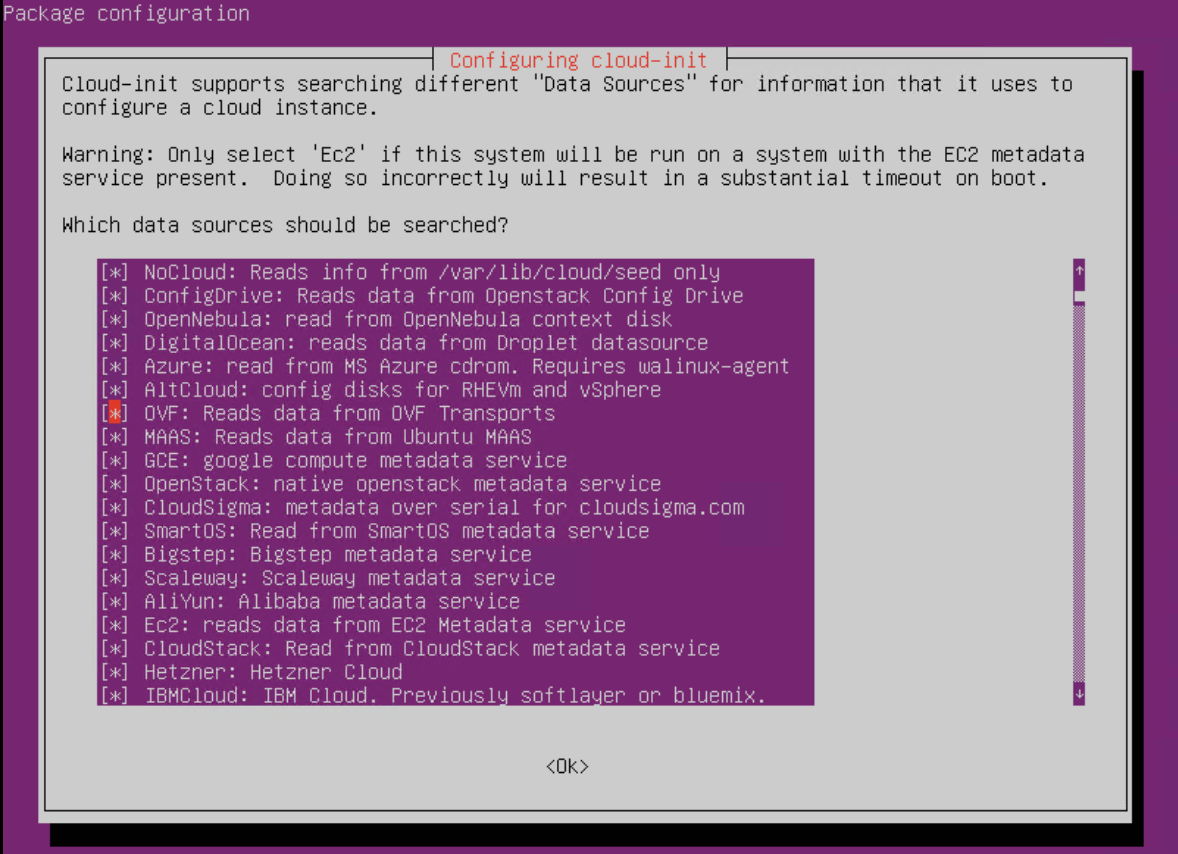
\includegraphics[width=0.4\textwidth]{imaxes/pruebaconcepto/vrealize/install-cloud-init.png}
    %         \caption{Configuración del servicio cloud-init en Ubuntu Server 20.}
    %         \label{fig:cloud-init-config}
    %     \end{figure}
    %     \FloatBarrier
    %     \begin{figure}[h]
    %         \centering
    %         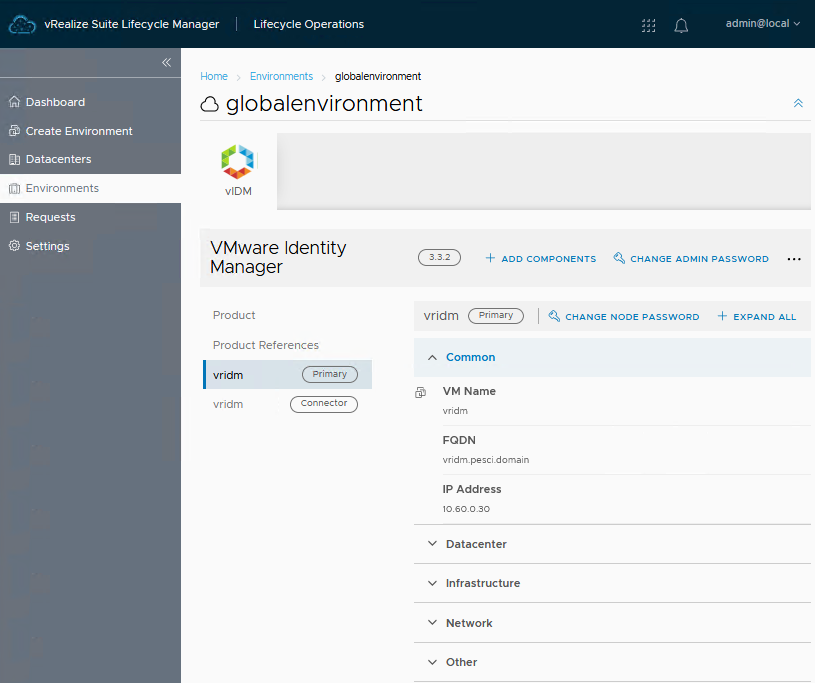
\includegraphics[width=0.4\textwidth]{imaxes/pruebaconcepto/vrealize/config-istance-vridm.png}
    %         \caption{Creación de una plantilla a partir de la VM de Ubuntu Server 20.}
    %         \label{fig:template-ubuntu}
    %     \end{figure}
    %     \FloatBarrier

    %     Una vez se tienen los recursos que serán usados por los usuarios es necesario añadirlos a vRA. Para poder esos recursos, durante su configuración vRA se asigna un tag a cada uno con la forma \textit{key:value}. En una blueprint estos tags permitirán indicar a que recurso se está refiriendo. 
    %     Lo primero es configurar una Cloud Zone que proporcionará acceso a todos los recursos situados en el cluster vSphere. El tag utilizado para esta será \textit{cloud:private}. Posteriormente se definen los tamaños de VMs que se habilitan, también llamado Flavour Mapping. Se configuran cuatro tamaños, X-small (1 CPU y 512 MB de RAM), Small (2 CPU y 8 GB de RAM), Medium (8 CPU y 4 GB de RAM) y Large (8 CPU y 16 GB de RAM). Las redes disponibles se añaden mediante la creación de perfiles donde se definen los tags con los que se identifica la red, su gateway, su servidor DNS, el rango de IPs para asignar una IP a cada VM conectada a esa red. 
\end{subsection}